\section{Full-wave Rectifier}
Mạch sau đây được gọi là bộ chỉnh lưu diode cầu toàn sóng. Cho máy biến áp có tỷ số N1/N2 = 10. Viết phương trình chênh lệch điện áp \(V_{AB}\) và \(V_{CD}\).
Sau đó, thực hiện phân tích miền thời gian (transient) để kiểm tra phương trình bạn đã viết.
\begin{figure}[ht]
    {\centering
    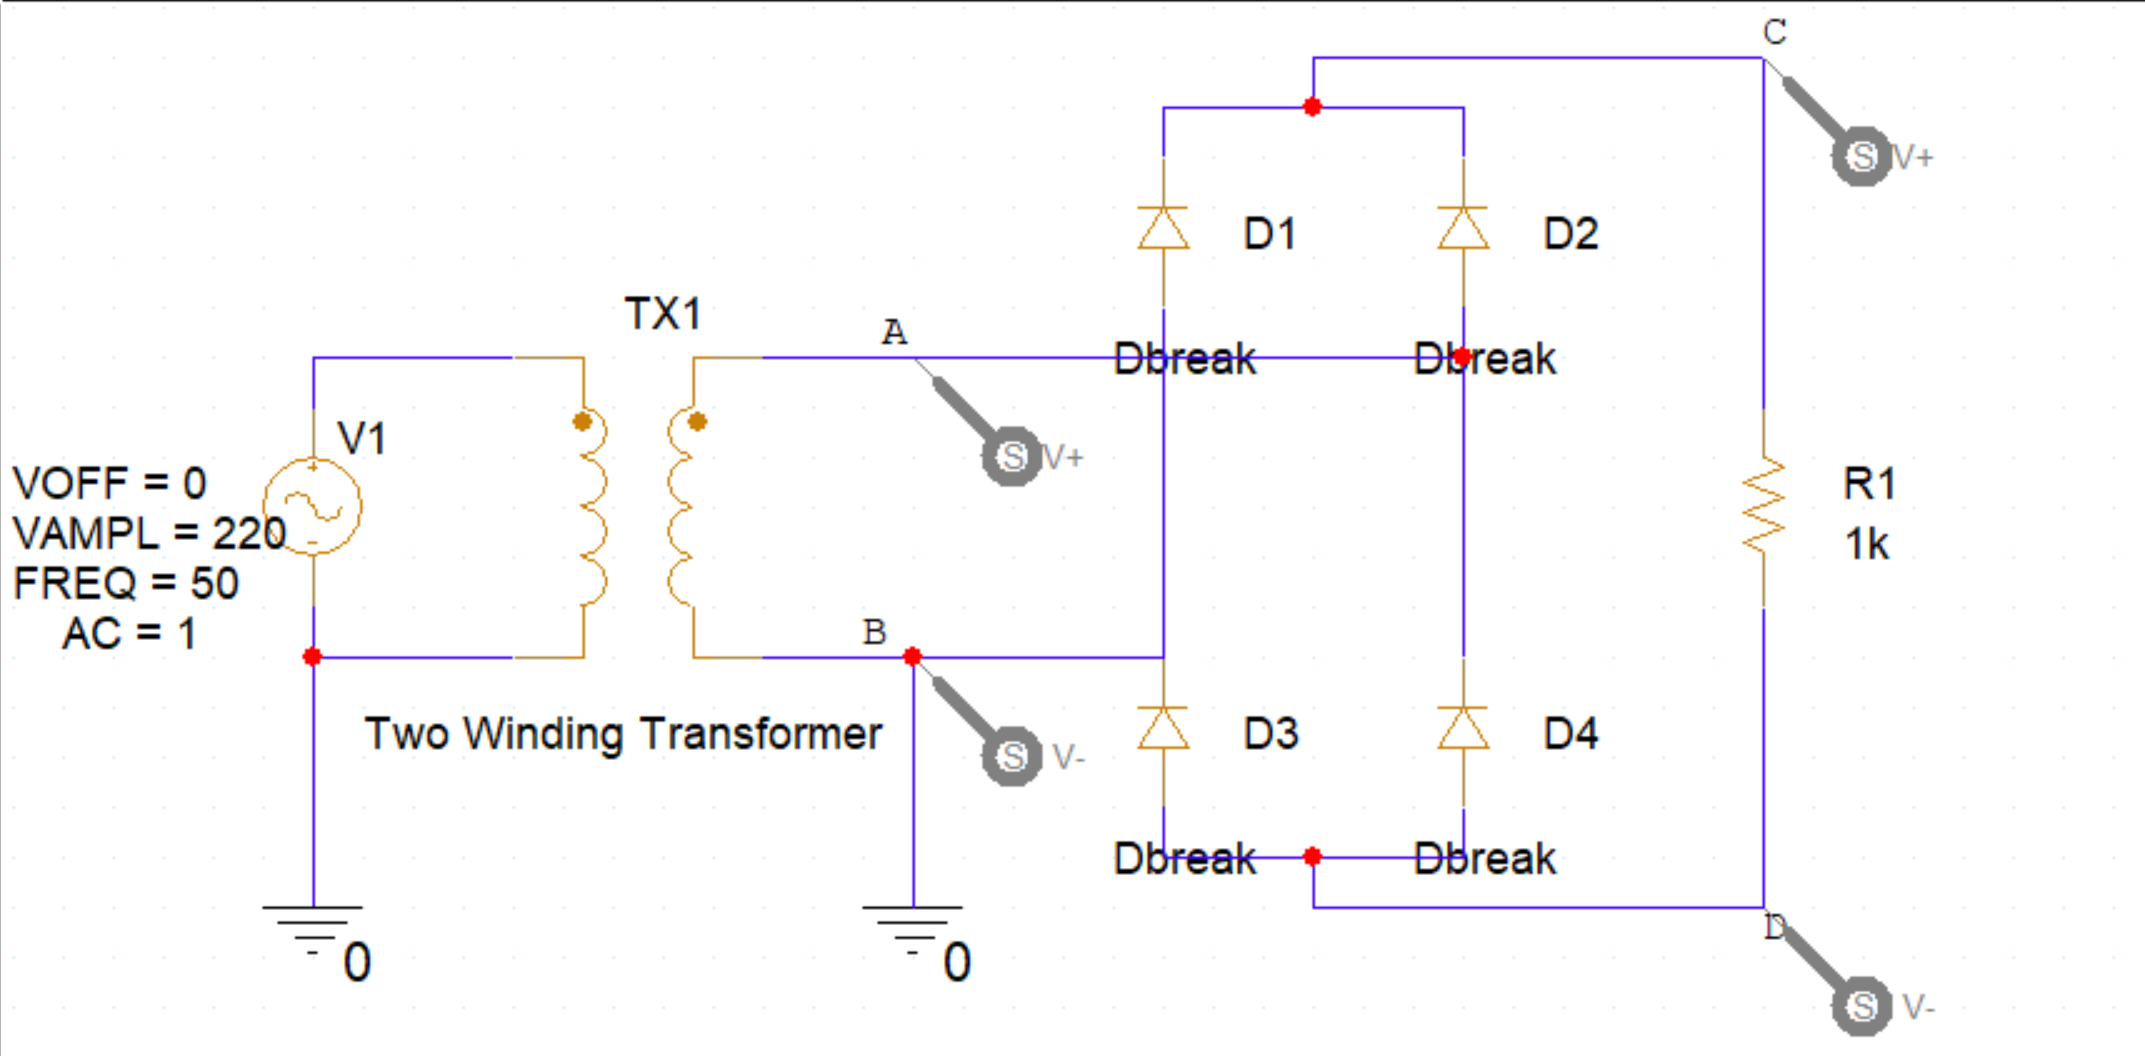
\includegraphics[scale=0.27]{graphics/ex7/f1.png}
    \caption{Full-wave bridge rectifier}}
\end{figure}
    \textbf{Tips 1:} Để dặt thành phần \textbf{transformer}: 
    \begin{itemize}
    \item \textbf{Step 1:} Đi tới \textbf{Place > PSpice Component > Modeling Application...}
    \item \textbf{Step 2:} Duyệt tìm thành phần \textbf{transformer} trong danh mục \textbf{System Modules} như trong hình sau: 
\begin{figure}[ht]
{\centering
    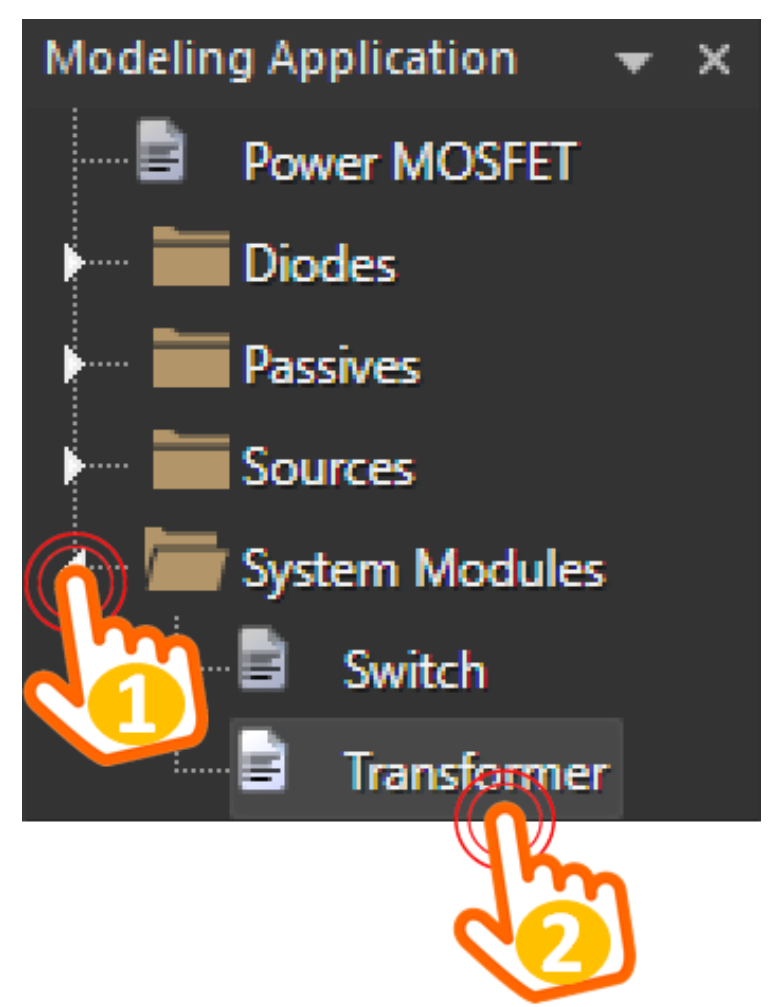
\includegraphics[scale=0.24]{graphics/ex7/f2.png}
    \caption{Duyệt tìm thành phần \textbf{transformer}}}
\end{figure}

    \item \textbf{Step 3:} Đặt tỷ lệ chuyển đổi trước khi đặt như hình dưới đây.


\begin{figure}[ht]
    
    {\centering
        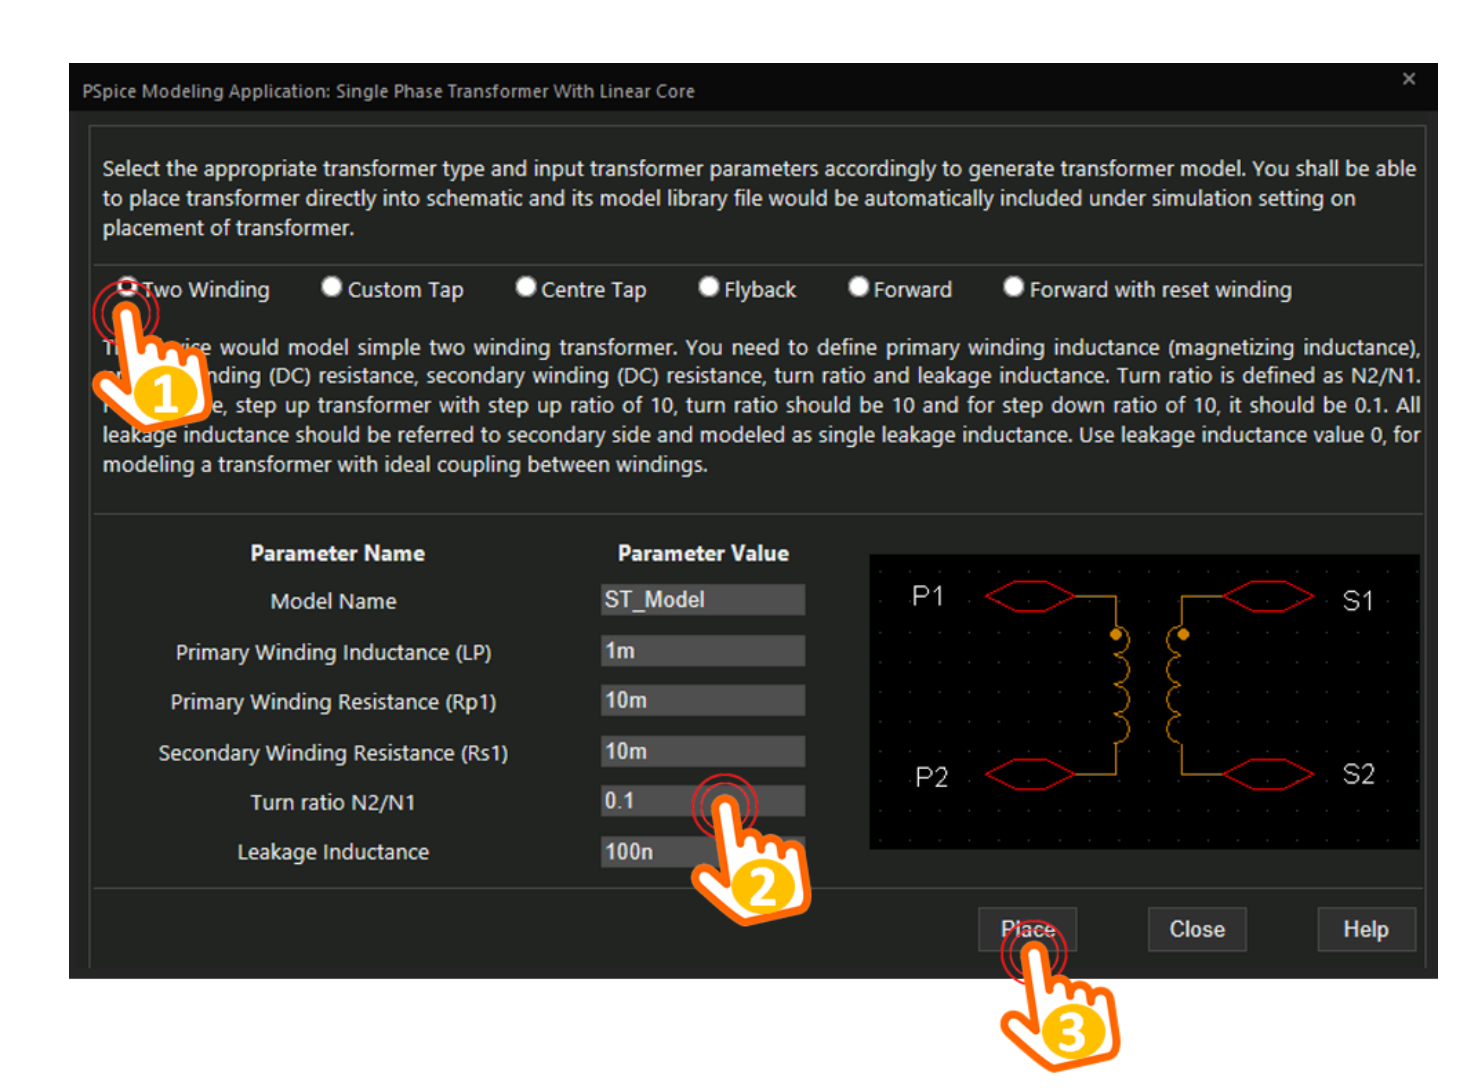
\includegraphics[scale=0.3]{graphics/ex7/f3.png}
        \caption{Thiết lập tỷ số biến đổi trước khi đặt máy biến áp}}
  
\end{figure}
\end{itemize}

\textbf{Tip 2:} Các điểm đánh dấu chênh lệch điện áp trong PSPICE cho TI:
\begin{figure}[h]
\centering
        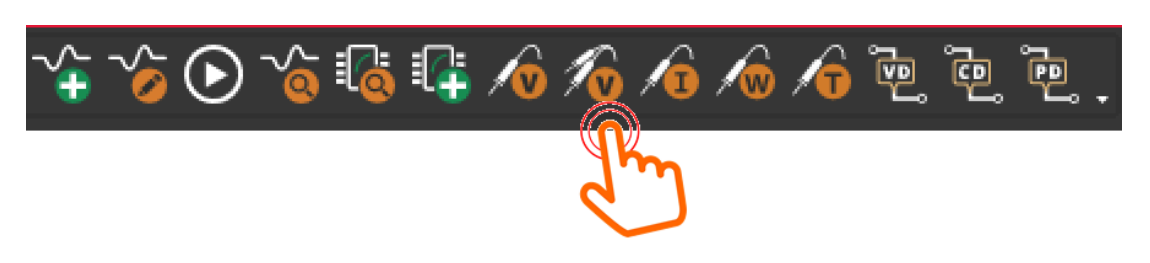
\includegraphics[scale=0.3]{graphics/ex7/f4.png}
        \caption{Các điểm đánh dấu chênh lệch điện áp trong PSPICE cho TI:}
\end{figure}
\newpage
\subsection{Tính toán theo lí thuyết}
\textbf{Ghi chú:}

Những giải thích, công thức và phương trình được mong đợi hơn là chỉ có kết quả.

\textbf{Xấp xỉ:} diodes có \(V_f = 0,7\) (V)
\begin{itemize}
    \item \(V_{AB} = \dfrac{N2}{N1}.V_1 = 0,1.220 = 22\) (V)
    \item \(V_{AB} - V_{D2} - V_{CD} - V_{D3} = 0\) hoặc \(V_{AB} - V_{D1} - V_{CD} - V_{D4} = 0\) (KVL)

\(\rightarrow V_{CD} = V_{AB} - 2.0,7 = 20,6 \) (V)
\end{itemize}

\subsection{Mô phỏng}
Dạng sóng hình sin của hiệu điện thế \(V_{AB}\) có chu kỳ T = 20 (ms)
Nếu chúng ta muốn thực hiện phân tích nhất thời trong 10 chu kỳ của dạng sóng \(V_{AB}\) thì thời gian cần thiết sẽ là: 200 (ms)

Nếu chúng ta muốn tốc độ lấy mẫu cao gấp 10 lần tần số của sóng hình sin
chênh lệch điện áp \(V_{AB}\), khoảng thời gian giữa hai thời điểm lấy mẫu liên tiếp
nên là: 2 (ms)



Bây giờ, hãy tạo một hồ sơ mô phỏng như hướng dẫn trong \textbf{Bài tập 3.6} và thực hiện mô phỏng của bạn để kiểm tra nó!



\textbf{Kết quả mô phỏng:} Hiển thị cả \(V_{AB}\) và \(V_{CD}\) trong một cửa sổ đồ thị để minh họa 
mối quan hệ giữa họ. Đừng quên sử dụng con trỏ để chứng minh rằng phương trình 
bạn đã viết là chính xác.

\begin{figure}[h]
    \centering
    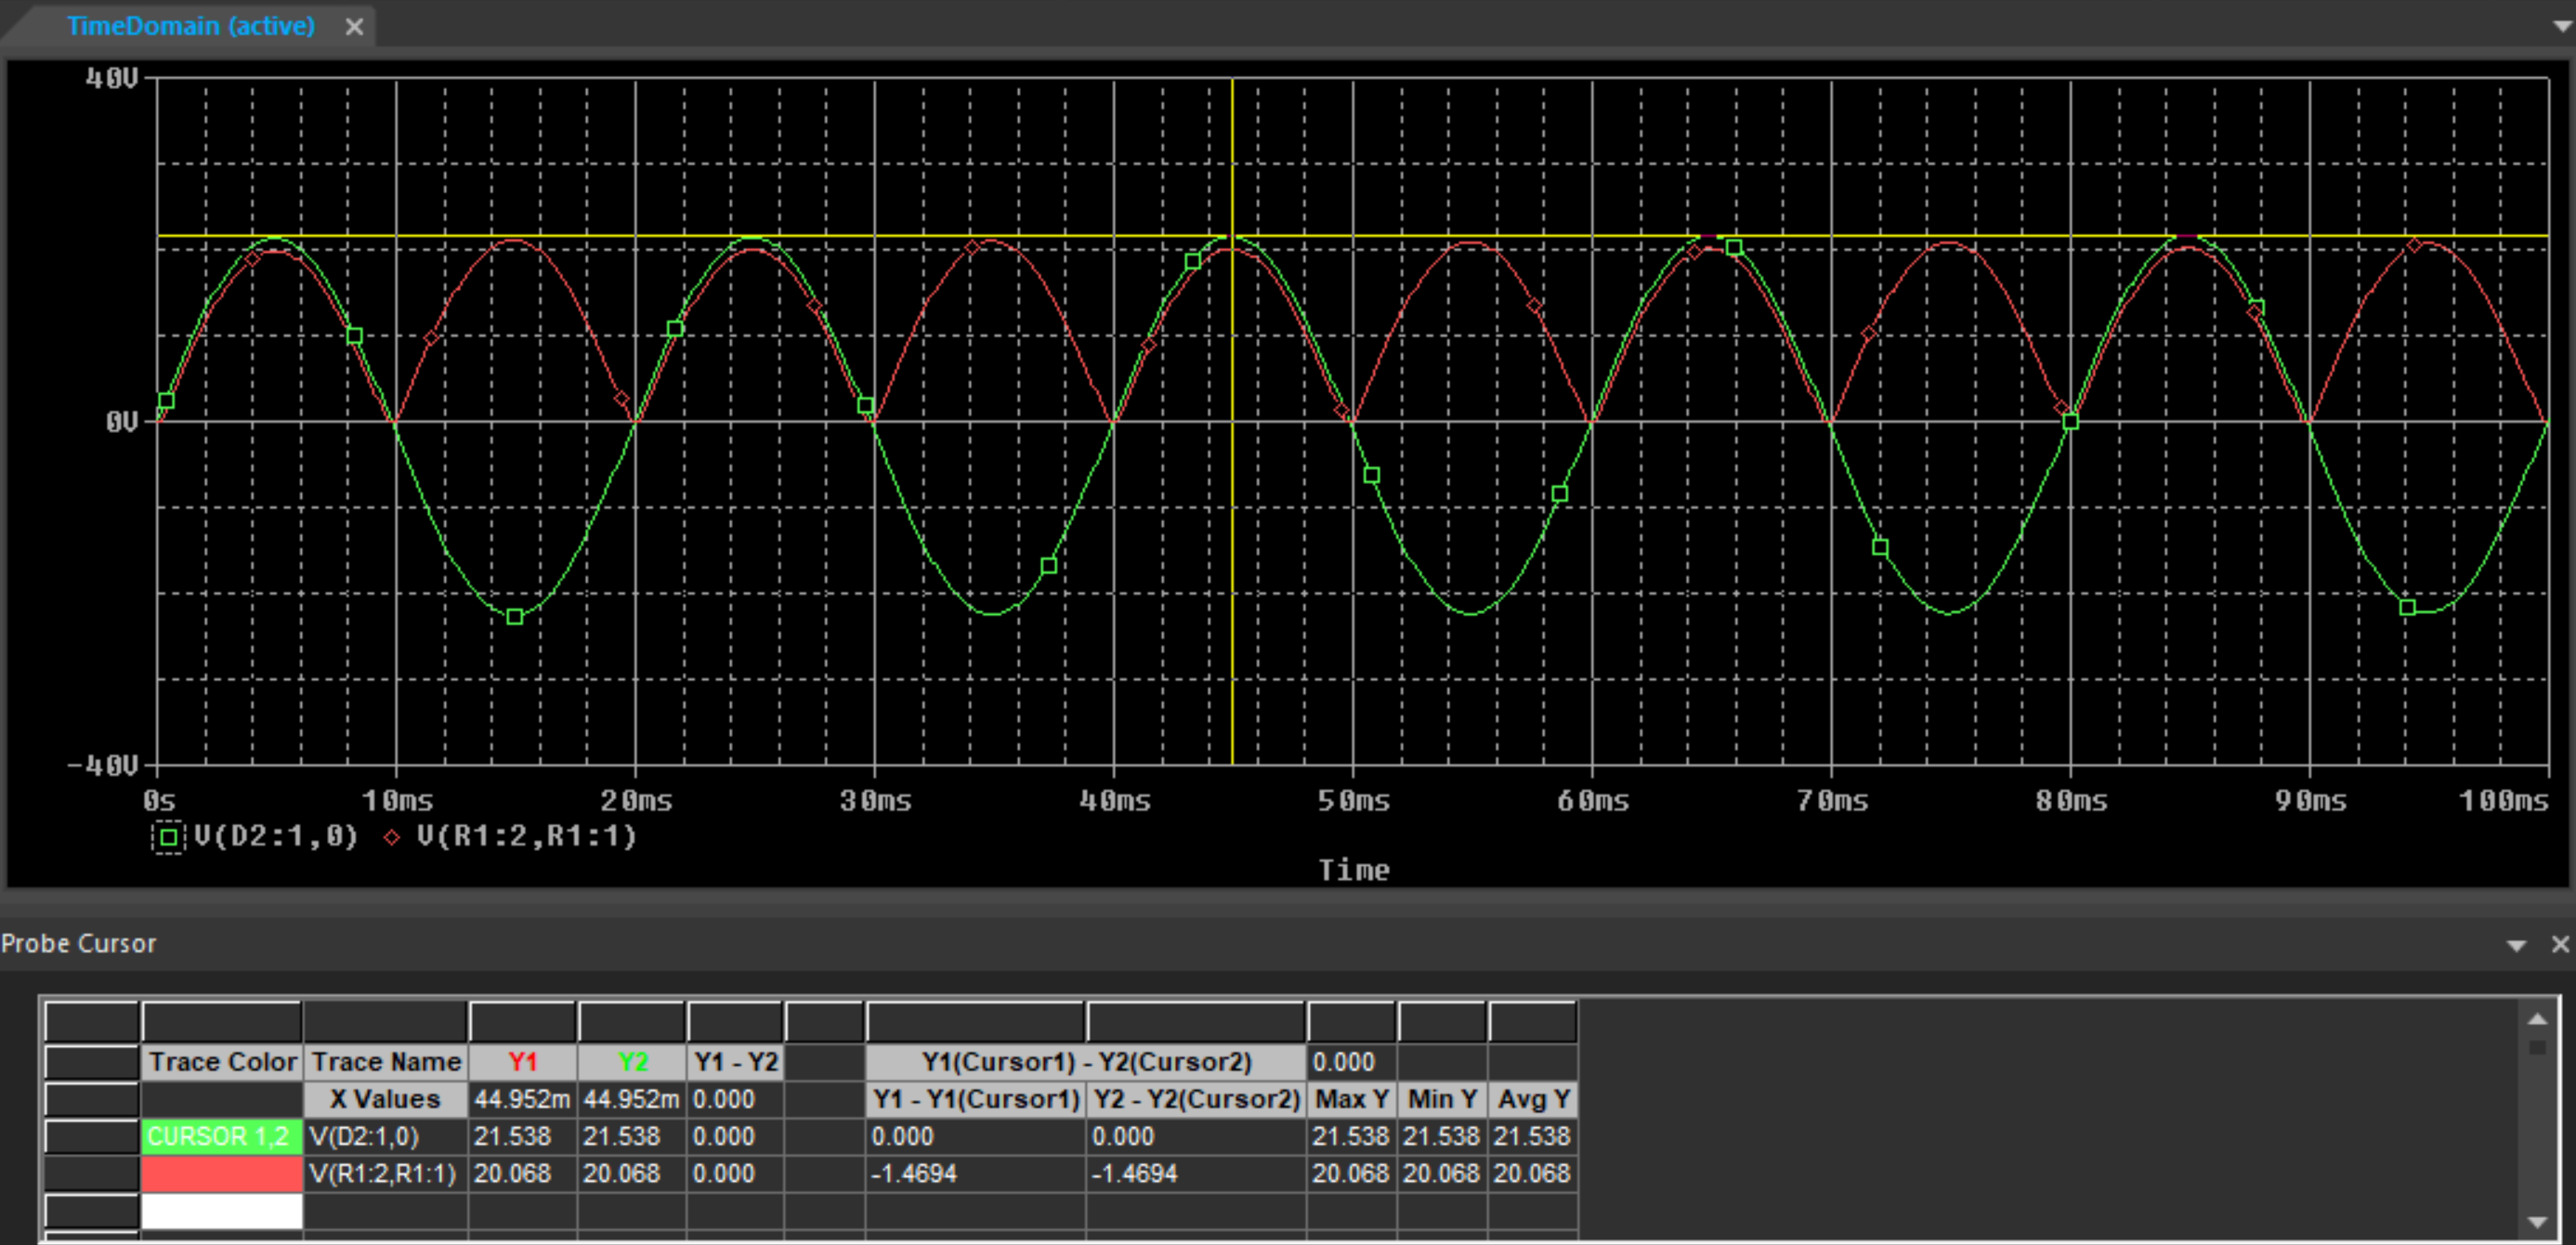
\includegraphics[scale=0.2]{graphics/ex7/f5.png}
\end{figure}





